\chapter{Diagramme der Auswertung}
In diesem Kapitel finden Sie Diagramme der Auswertungen zu den im Methodologieteil gestellten Fragen. Einzelne, aus unserer Sicht, relevante Diagramme sind hier nicht aufgef�hrt, da diese direkt im Kapitel <<Ergebnisse / Resultate>> abgebildet wurden.

\begin{figure}[h]
	\centering
		
	\ifpdf
		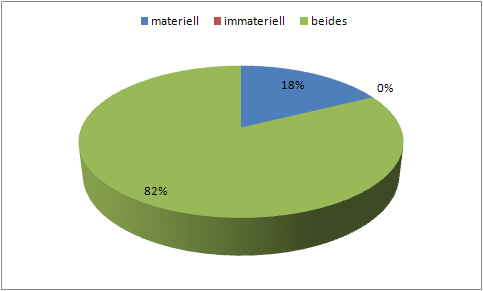
\includegraphics[width=0.9\textwidth]{chap12-unternehmen-anreizmix.png}
	\else	
		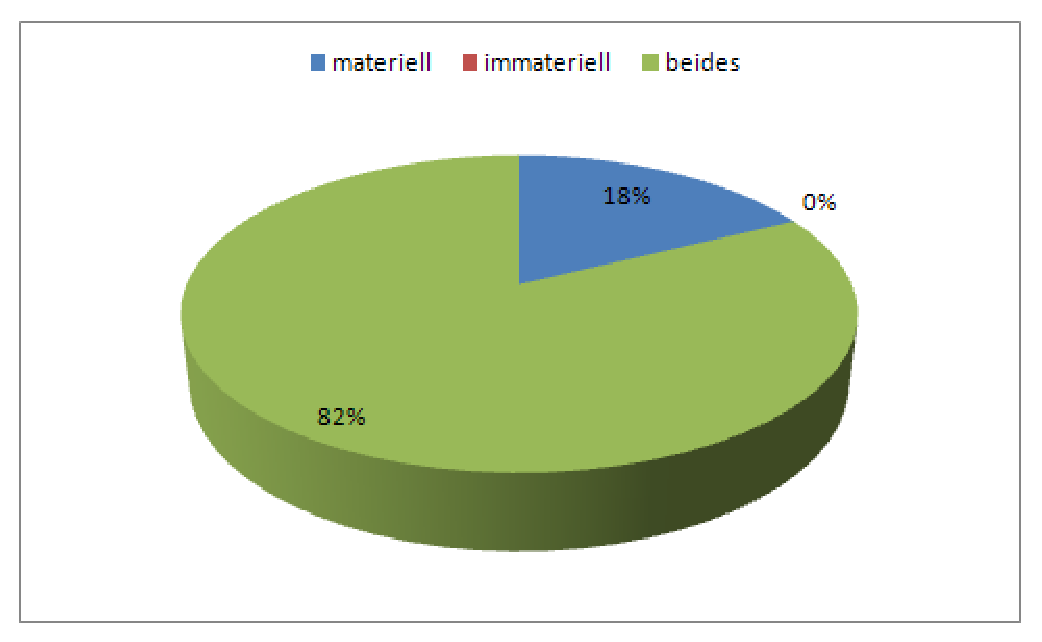
\includegraphics[width=0.9\textwidth]{chap12-unternehmen-anreizmix.eps}
	\fi
		
	\caption[Anreizmix aus Sicht von Unternehmen]{Anreizmix aus Sicht von Unternehmen (Eigene Darstellung)}	
	\label{fig:anreizMixUnternehmen}
\end{figure}

\begin{figure}[h]
	\centering
		
	\ifpdf
		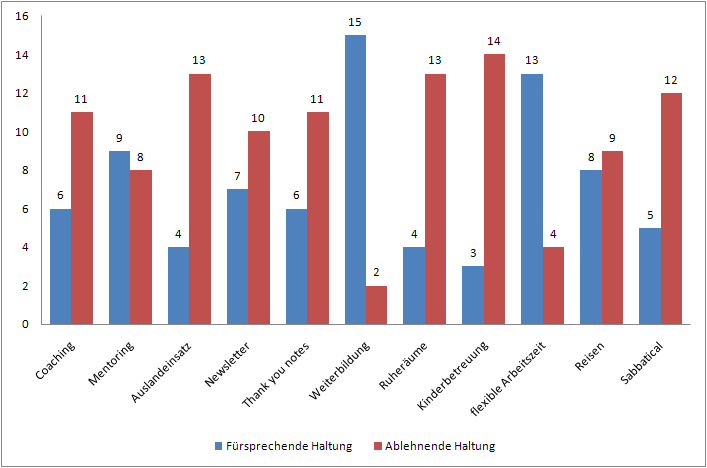
\includegraphics[width=0.9\textwidth]{chap12-unternehmen-proUndContra.png}
	\else	
		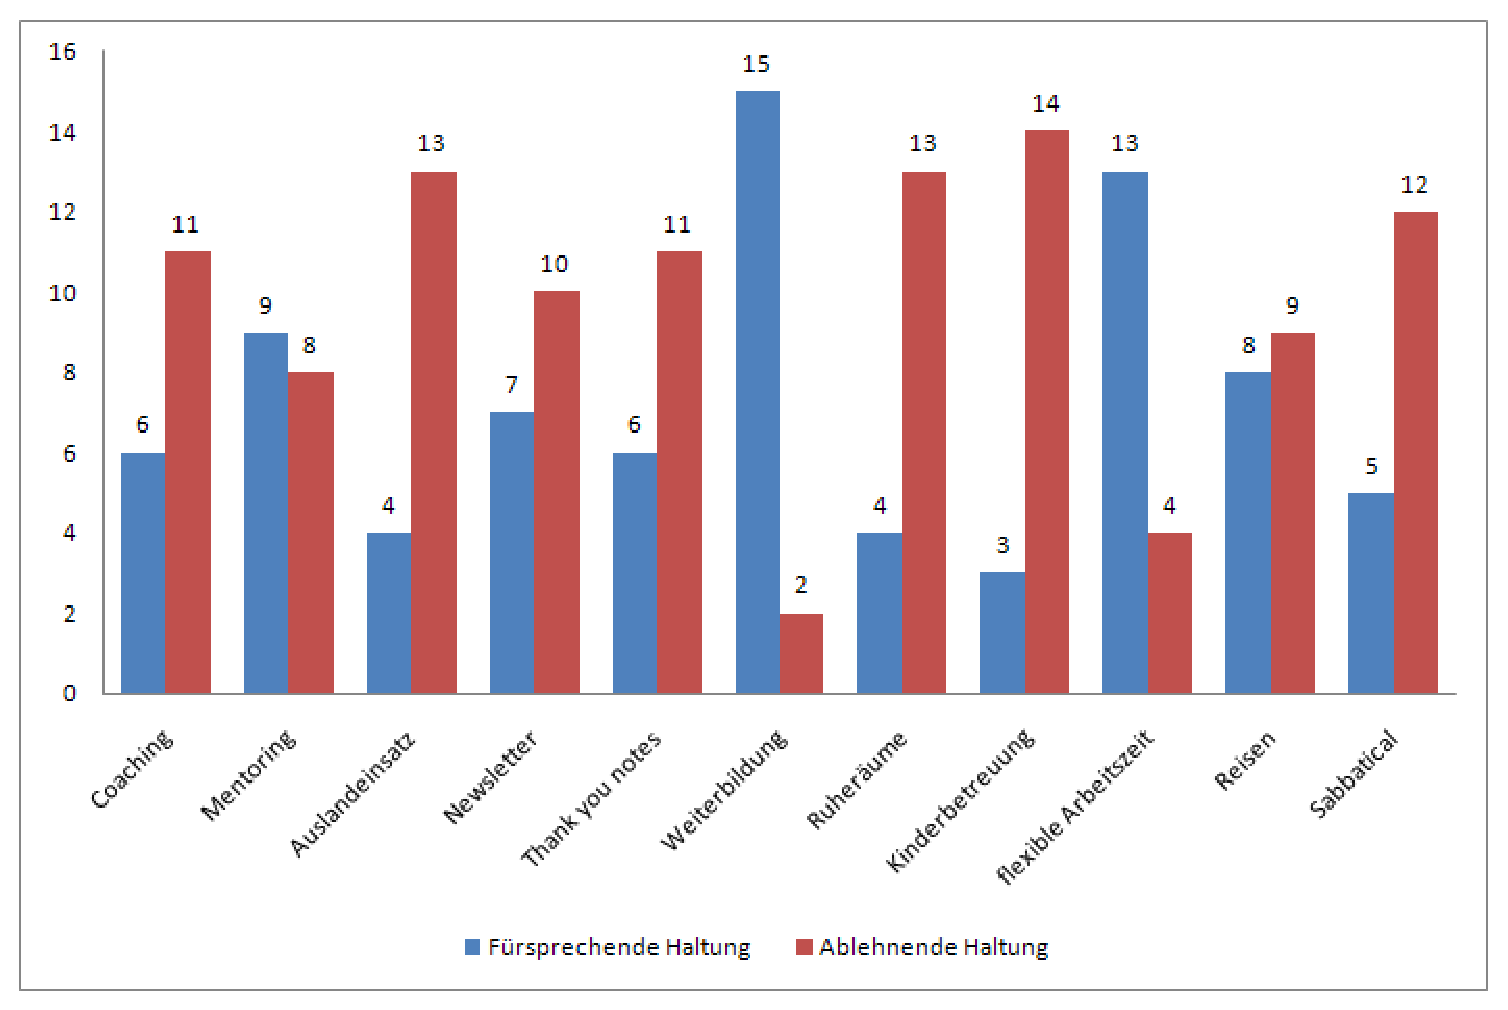
\includegraphics[width=0.9\textwidth]{chap12-unternehmen-proUndContra.eps}
	\fi
		
	\caption[Haltungen zu immaterielle Anreizen]{Haltungen zu immaterielle Anreizen (Eigene Darstellung)}	
	\label{fig:anreizHaltungUnternehmen}
\end{figure}

\begin{figure}[h]
	\centering
		
	\ifpdf
		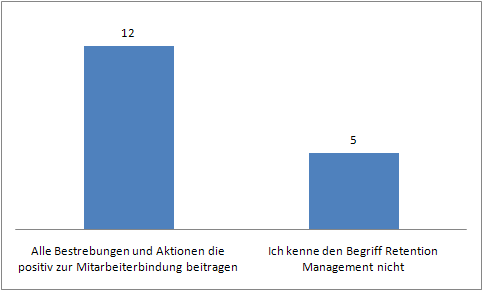
\includegraphics[width=0.9\textwidth]{chap12-unternehmen-retentionmanagement.png}
	\else	
		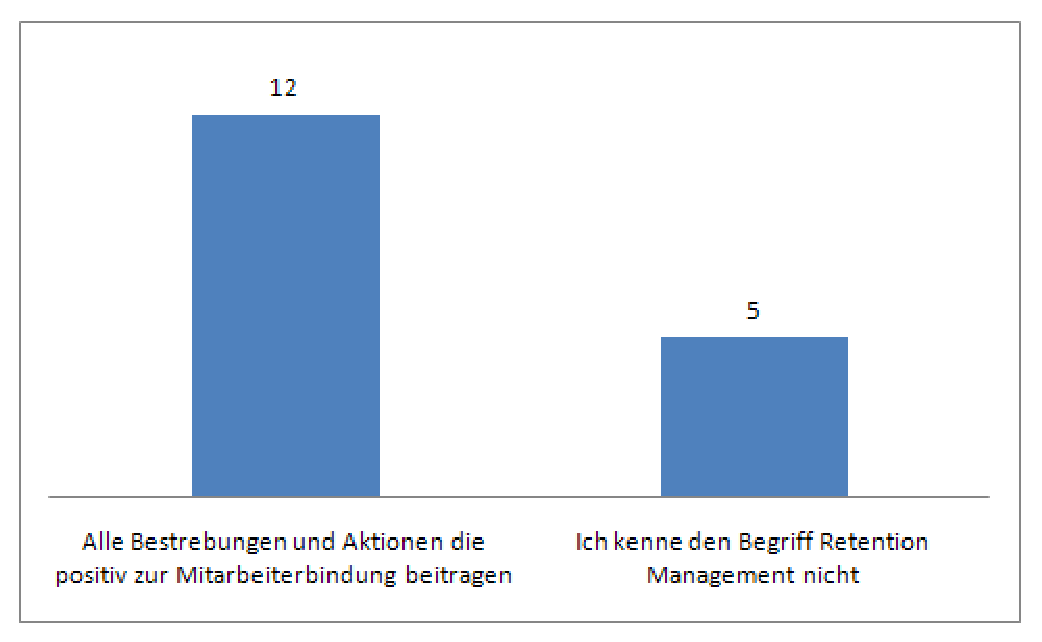
\includegraphics[width=0.9\textwidth]{chap12-unternehmen-retentionmanagement.eps}
	\fi
		
	\caption[Verst�ndnis von Retention Management]{Verst�ndnis von Retention Management (Eigene Darstellung)}	
	\label{fig:whatIsRetention}
\end{figure}

\begin{figure}[h]
	\centering
		
	\ifpdf
		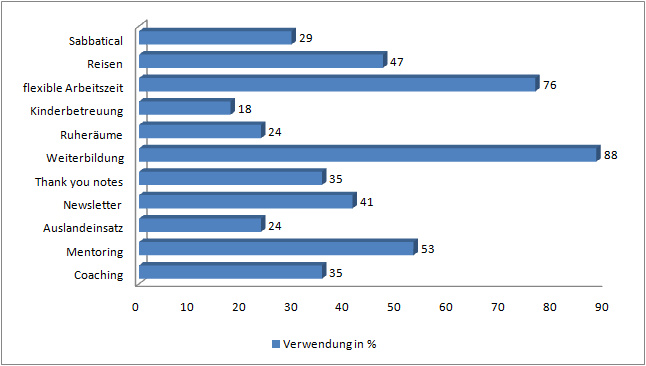
\includegraphics[width=0.9\textwidth]{chap12-unternehmen-anreizverwendung.png}
	\else	
		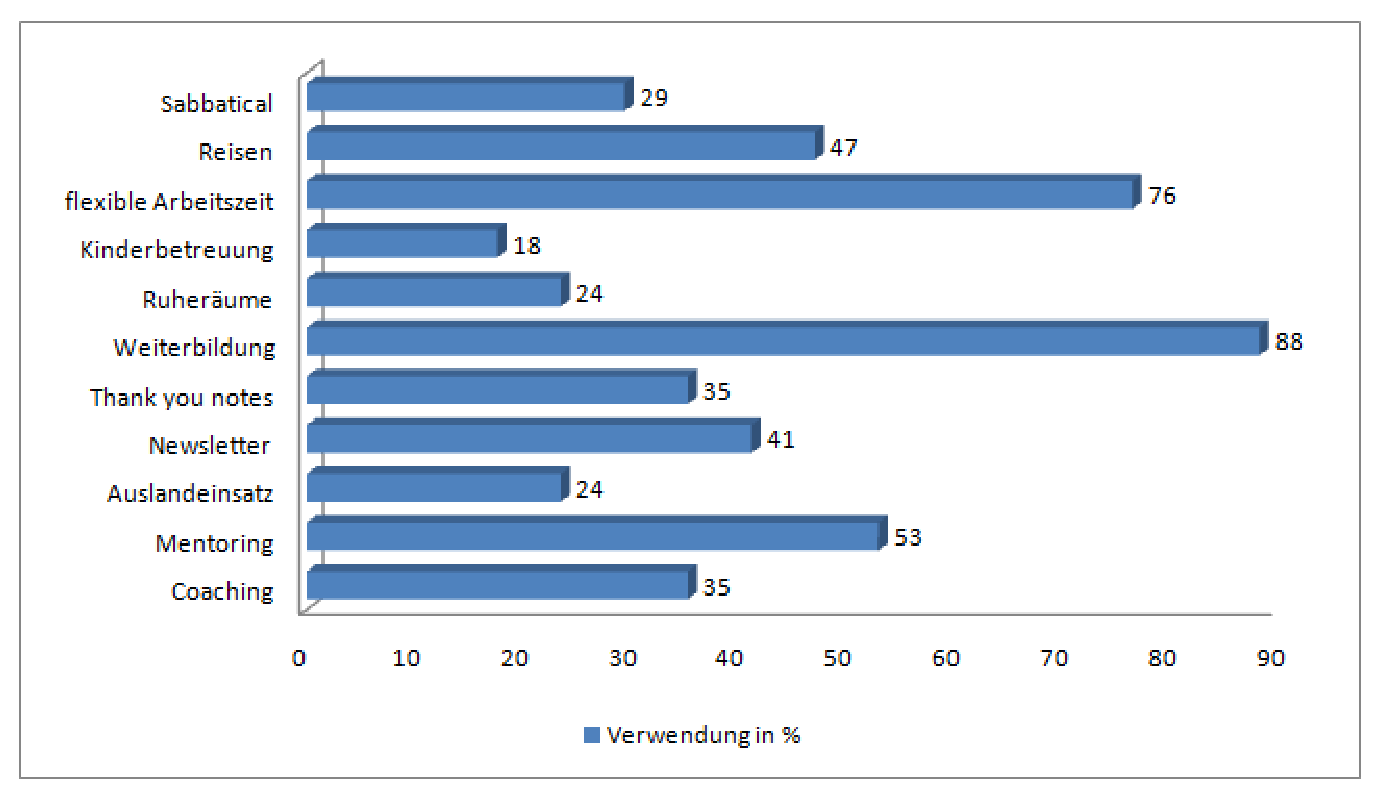
\includegraphics[width=0.9\textwidth]{chap12-unternehmen-anreizverwendung.eps}
	\fi
		
	\caption[Prozentualer Einsatz von Anreizen]{Prozentualer Einsatz von Anreizen (Eigene Darstellung)}	
	\label{fig:usageInPercentage}
\end{figure}